% Matemàtiques II — Notes de Classe (estil «Apunts de Física II»)
% Compilar:  cd latex/mates && python3 ../../tools/md2tex.py && pdflatex main && pdflatex main
\documentclass[a4paper,10pt]{article}
\usepackage[utf8]{inputenc}
\usepackage[provide=*,main=catalan]{babel}
\usepackage{amsmath,amssymb,booktabs,tabularx,graphicx,float,eurosym,textcomp,array}
\usepackage{pdflscape}
\usepackage[hidelinks,bookmarksnumbered]{hyperref}
\usepackage[a4paper,left=64.6pt,textwidth=480pt,top=62pt,textheight=672pt]{geometry}
\setlength{\parindent}{0pt}
\setlength{\parskip}{5pt plus 1pt minus 1pt}
\setlength{\abovecaptionskip}{8pt}
\renewcommand{\arraystretch}{1.15}
\providecommand{\euro}{\texteuro}
\newcommand{\D}[1]{\ensuremath{\displaystyle #1}}
\DeclareMathOperator{\sen}{sen}
\DeclareMathOperator{\tg}{tg}
\usepackage{needspace}
\raggedbottom
\widowpenalty=10000 \clubpenalty=10000
\let\oldsection\section\renewcommand{\section}{\needspace{7\baselineskip}\oldsection}
\let\oldsubsection\subsection\renewcommand{\subsection}{\needspace{5\baselineskip}\oldsubsection}
\renewcommand{\topfraction}{0.9}\renewcommand{\bottomfraction}{0.8}\renewcommand{\textfraction}{0.1}\renewcommand{\floatpagefraction}{0.75}
\setlength{\textfloatsep}{14pt plus 3pt minus 3pt}\setlength{\intextsep}{12pt plus 3pt minus 3pt}
\setcounter{tocdepth}{0}
\renewcommand{\thesection}{\arabic{section}.}
\renewcommand{\thesubsection}{\arabic{section}.\arabic{subsection}.}
\renewcommand{\thesubsubsection}{\arabic{section}.\arabic{subsection}.\arabic{subsubsection}.}
\renewcommand{\contentsname}{}

% ---- entrades de l'índex (blocs en negreta, temes dins del bloc)
\makeatletter
\def\l@bloc#1#2{\addpenalty{-\@highpenalty}\vskip 1.4em plus 1pt\@dottedtocline{0}{0em}{4.6em}{\bfseries #1}{\bfseries #2}}
\def\l@tema#1#2{\@dottedtocline{0}{1.2em}{3.4em}{#1}{#2}}
\def\l@annex#1#2{\@dottedtocline{0}{1.2em}{3.4em}{#1}{#2}}
\makeatother

\newcounter{blocn}\newcounter{temaid}
\renewcommand{\theHsection}{\arabic{temaid}.\arabic{section}}
\renewcommand{\theHequation}{\arabic{temaid}.\arabic{equation}}
\makeatletter\def\toclevel@bloc{0}\def\toclevel@tema{0}\def\toclevel@annex{0}\makeatother
\newcommand{\blankpage}{\clearpage\thispagestyle{empty}\mbox{}\clearpage}
\newcommand{\cleartoodd}{\clearpage\ifodd\value{page}\else\thispagestyle{empty}\mbox{}\clearpage\fi}
\newcommand{\cleartoeven}{\clearpage\ifodd\value{page}\thispagestyle{empty}\mbox{}\clearpage\fi}
\newcommand{\bloc}[3]{% número, títol, descripció (+ llista de temes a #4 via \blocllista)
  \cleartoodd\refstepcounter{blocn}
  \phantomsection\addcontentsline{toc}{bloc}{\protect\numberline{Bloc \theblocn.}#2}
  \thispagestyle{empty}
  \vspace*{0.28\textheight}
  \begin{center}
    {\Large\bfseries Bloc #1}\\[1.2em]
    {\Huge\bfseries #2}\\[1.6em]
    \begin{minipage}{0.7\textwidth}\centering\large #3\end{minipage}
  \end{center}
  \vspace{2.2em}\blocllista}
\newcommand{\blocllista}{}
\newcommand{\blocitems}[1]{\renewcommand{\blocllista}{\begin{center}\begin{minipage}{0.62\textwidth}#1\end{minipage}\end{center}}}

\newcommand{\tema}[2]{% número, títol
  \cleartoodd\stepcounter{temaid}
  \setcounter{section}{0}\setcounter{equation}{0}
  \phantomsection\addcontentsline{toc}{tema}{\protect\numberline{#1.}#2}
  \begin{center}
    {\LARGE\bfseries Tema #1: #2}\\[1.1em]
    {\large Lucas Granado}\\[0.7em]
    {\large 4 de novembre de 2026}
  \end{center}
  \vspace{1.2em}}
\newcommand{\annex}[2]{% lletra, títol
  \clearpage\stepcounter{temaid}
  \setcounter{section}{0}\setcounter{equation}{0}
  \phantomsection\addcontentsline{toc}{annex}{\protect\numberline{#1.}#2}
  \begin{center}
    {\LARGE\bfseries Annex #1: #2}\\[1.1em]
    {\large Lucas Granado}
  \end{center}
  \vspace{1.2em}}

\pagestyle{empty}
\renewcommand{\cleartoodd}{\clearpage}
\begin{document}
\pagestyle{empty}
% ---------------------------------------------------------------- Bloc 3
\blocitems{\begin{itemize}\item Tema 6. Vectors a l'espai\item Tema 9. Equacions de rectes i plans\item Tema 10. Posició relativa de rectes i plans\item Tema 11. Distàncies i angles\end{itemize}}
\bloc{3}{Geometria a l'espai}{Vectors, rectes i plans, posicions relatives, distàncies i angles.}
\tema{6}{Vectors a l'espai}\section{Localització dels punts a l'espai}

Per localitzar punts a l'espai tridimensional s'utilitza un \textbf{sistema de referència cartesià} format per tres rectes perpendiculars entre si que s'anomenen \textbf{eixos de coordenades}, designats per $x$, $y$ i $z$. Qualsevol punt de l'espai queda determinat per tres coordenades $(x, y, z)$.

\begin{figure}[H]
\centering
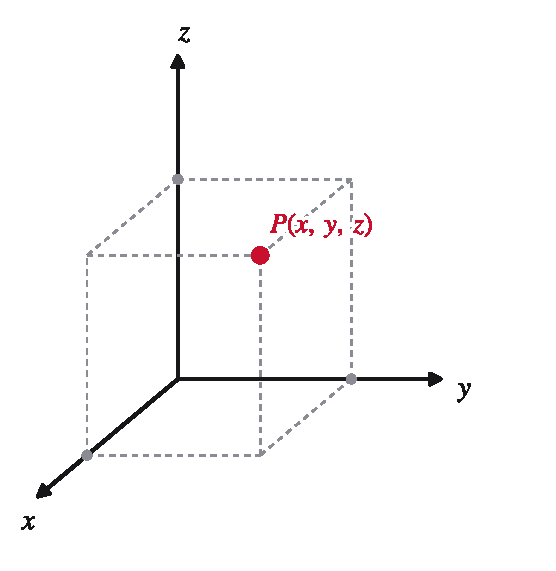
\includegraphics[width=267pt]{fig/m06_f14.pdf}
\caption{Sistema de coordenades cartesianes a l'espai: qualsevol punt $P$ queda determinat per la terna $(x, y, z)$.}
\end{figure}

\section{Components d'un vector a l'espai}

\textbf{Definició:} Els \textbf{components} d'un vector s'obtenen restant ordenadament les coordenades del seu extrem menys les del seu origen. Donats els punts $A(a_1, a_2, a_3)$ i $B(b_1, b_2, b_3)$, el vector $\overrightarrow{AB}$ té components:

\begin{equation}
\overrightarrow{AB} = (b_1 - a_1,\; b_2 - a_2,\; b_3 - a_3)
\end{equation}

Per definir un vector calen tres elements: \textbf{direcció}, \textbf{sentit} i \textbf{magnitud} (mòdul).

Si el vector $\overrightarrow{AB}$ té la mateixa longitud, direcció i sentit que un altre vector $\overrightarrow{CD}$, es tracta de dos vectors \textbf{equipol\textperiodcentered{}lents}. El conjunt de tots els vectors fixos equipol\textperiodcentered{}lents s'anomena \textbf{vector lliure}.

\subsection{Mòdul d'un vector}

El mòdul d'un vector $\vec v = (v_1, v_2, v_3)$ és la seva longitud:

\begin{equation*}
|\vec v| = \sqrt{v_1^2 + v_2^2 + v_3^2}
\end{equation*}

\subsection{Vector unitari}

El vector unitari en la direcció de $\vec v$ és aquell de mòdul 1:

\begin{equation*}
\hat u_v = \frac{\vec v}{|\vec v|}
\end{equation*}

\section{Operacions amb vectors}

\subsection{Suma de vectors}

Donats $\vec a = (a_1, a_2, a_3)$ i $\vec b = (b_1, b_2, b_3)$, el seu vector suma és:

\begin{equation*}
\vec a + \vec b = (a_1 + b_1,\; a_2 + b_2,\; a_3 + b_3)
\end{equation*}

La suma de vectors compleix les propietats següents:

\begin{itemize}
\item \textbf{Commutativa:} $\vec a + \vec b = \vec b + \vec a$
\item \textbf{Associativa:} $\vec a + (\vec b + \vec c) = (\vec a + \vec b) + \vec c$
\item \textbf{Element neutre:} el vector nul $\vec 0 = (0, 0, 0)$ compleix $\vec a + \vec 0 = \vec a$
\item \textbf{Element simètric:} cada vector $\vec a$ té un oposat $-\vec a$ tal que $\vec a + (-\vec a) = \vec 0$
\end{itemize}

\subsection{Multiplicació d'un vector per un escalar}

Donat $k \in \mathbb{R}$ i $\vec a = (a_1, a_2, a_3)$:

\begin{equation*}
k\cdot\vec a = (k a_1,\; k a_2,\; k a_3)
\end{equation*}

Propietats:

\begin{itemize}
\item $k\cdot(\vec a + \vec b) = k\vec a + k\vec b$
\item $1\cdot\vec a = \vec a$
\item $(k + h)\cdot\vec a = k\vec a + h\vec a$
\item $(k\cdot h)\cdot\vec a = k\,(h\cdot\vec a)$
\end{itemize}

\section{Combinació lineal de vectors}

\textbf{Definició:} Donat un conjunt de vectors $\vec v_1, \vec v_2, \vec v_3$ d'un espai vectorial, s'anomena \textbf{combinació lineal} d'aquests vectors tota expressió de la forma

\begin{equation}
\lambda_1\vec v_1 + \lambda_2\vec v_2 + \lambda_3\vec v_3 + \cdots
\end{equation}

on $\lambda_1, \lambda_2, \lambda_3, \ldots \in \mathbb{R}$.

Un vector $\vec v$ és combinació lineal de $\vec v_1, \vec v_2, \vec v_3$ si existeixen $\lambda_1, \lambda_2, \lambda_3$ que verifiquen l'expressió anterior.

\section{Dependència i independència lineal de vectors}

Els vectors $\vec v_1, \vec v_2, \vec v_3$ són \textbf{linealment independents} si l'única solució de

\begin{equation*}
\lambda_1\vec v_1 + \lambda_2\vec v_2 + \lambda_3\vec v_3 = \vec 0
\end{equation*}

és $\lambda_1 = \lambda_2 = \lambda_3 = 0$. En cas contrari, és a dir, si existeix alguna solució amb algun $\lambda_i \neq 0$, els vectors són \textbf{linealment dependents} (un d'ells és combinació lineal dels altres).

\section{Producte escalar de dos vectors}

\textbf{Definició:} El \textbf{producte escalar} de dos vectors $\vec a$ i $\vec b$ és el nombre real

\begin{equation}
\vec a\cdot\vec b = |\vec a|\,|\vec b|\cos\alpha
\end{equation}

on $\alpha$ és l'angle que formen els dos vectors. En components, si $\vec a = (a_1, a_2, a_3)$ i $\vec b = (b_1, b_2, b_3)$:

\begin{equation}
\vec a\cdot\vec b = a_1b_1 + a_2b_2 + a_3b_3
\end{equation}

\subsection{Propietats geomètriques del producte escalar}

La figura següent il\textperiodcentered{}lustra les tres situacions principals:

\begin{figure}[H]
\centering
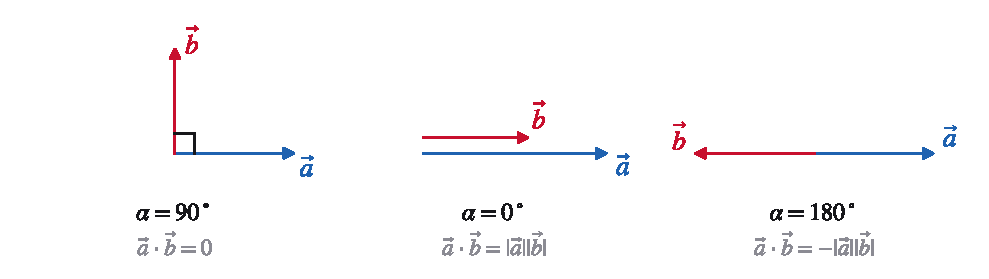
\includegraphics[width=372pt]{fig/m06_f15.pdf}
\caption{Interpretació geomètrica del producte escalar: perpendiculars ($\alpha = 90^\circ$), paral\textperiodcentered{}lels mateix sentit ($\alpha = 0^\circ$) i paral\textperiodcentered{}lels sentit contrari ($\alpha = 180^\circ$).}
\end{figure}

Les propietats geomètriques principals del producte escalar són:

\begin{enumerate}
\item \textbf{Angle entre dos vectors:}
\end{enumerate}

\begin{equation*}
\cos\alpha = \frac{\vec a\cdot\vec b}{|\vec a|\,|\vec b|} \;\Rightarrow\; \alpha = \arccos\!\left(\frac{\vec a\cdot\vec b}{|\vec a|\,|\vec b|}\right)
\end{equation*}

\begin{enumerate}
\item \textbf{Vectors perpendiculars o ortogonals:} $\vec a \perp \vec b$ si i només si $\vec a\cdot\vec b = 0$.
\end{enumerate}

\tema{9}{Equacions de rectes i plans}\section{La recta}

Una recta $r$ queda determinada per qualsevol d'aquestes dades:

\begin{itemize}
\item Dos punts $P$ i $Q$, o equivalentment un punt $P$ i el vector director $\vec u = \overrightarrow{PQ}$.
\item Dos plans $\pi_1$ i $\pi_2$ no paral\textperiodcentered{}lels (la recta és la seva intersecció).
\item Un punt $P$ i un pla $\pi$ perpendicular a la recta.
\end{itemize}

La figura il\textperiodcentered{}lustra els tres casos:

\begin{figure}[H]
\centering
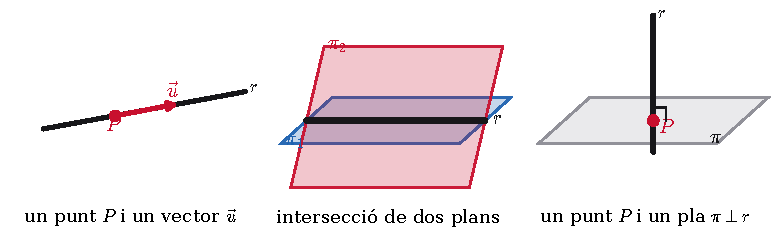
\includegraphics[width=372pt]{fig/m09_f17.pdf}
\caption{Tres maneres de determinar una recta a l'espai.}
\end{figure}

\subsection{Equació vectorial d'una recta}

Donat un punt $P(x_0, y_0, z_0)$ i un vector director $\vec u = (u_1, u_2, u_3)$:

\begin{equation*}
\vec x = \vec p + \lambda\,\vec u, \qquad \forall\lambda\in\mathbb{R}
\end{equation*}

\subsection{Equacions paramètriques d'una recta}

\begin{equation*}
\begin{cases} x = x_0 + \lambda\,u_1 \\ y = y_0 + \lambda\,u_2 \\ z = z_0 + \lambda\,u_3 \end{cases} \qquad \forall\lambda\in\mathbb{R}
\end{equation*}

\subsection{Equacions contínues d'una recta}

Aïllant $\lambda$ de les equacions paramètriques i igualant:

\begin{equation*}
\frac{x - x_0}{u_1} = \frac{y - y_0}{u_2} = \frac{z - z_0}{u_3}
\end{equation*}

\section{El pla}

Un pla $\pi$ queda determinat per qualsevol d'aquestes dades:

\begin{itemize}
\item Tres punts $P$, $Q$ i $R$ no alineats.
\item Un punt $P$ i dos vectors $\vec u$ i $\vec v$ linealment independents (vectors directors del pla).
\item Un punt $P$ i un vector $\vec n \neq \vec 0$ perpendicular al pla (vector normal).
\end{itemize}

\subsection{Equació vectorial d'un pla}

\begin{equation*}
\vec x = \vec p + \lambda\,\vec u + \mu\,\vec v, \qquad \forall\,\lambda,\mu\in\mathbb{R}
\end{equation*}

\subsection{Equacions paramètriques d'un pla}

\begin{equation*}
\begin{cases} x = x_0 + \lambda\,u_1 + \mu\,v_1 \\ y = y_0 + \lambda\,u_2 + \mu\,v_2 \\ z = z_0 + \lambda\,u_3 + \mu\,v_3 \end{cases} \qquad \forall\,\lambda,\mu\in\mathbb{R}
\end{equation*}

\subsection{Equació general (cartesiana) d'un pla}

S'obté desenvolupant el determinant de l'equació vectorial. La forma és:

\begin{equation*}
\begin{vmatrix} x - x_0 & u_1 & v_1 \\ y - y_0 & u_2 & v_2 \\ z - z_0 & u_3 & v_3 \end{vmatrix} = 0 \;\Longrightarrow\; Ax + By + Cz + D = 0
\end{equation*}

\section{Vector associat a un pla}

Donat el pla $\pi: Ax + By + Cz + D = 0$, el vector $\vec n = (A, B, C)$ és perpendicular al pla i s'anomena \textbf{vector normal} o \textbf{vector associat}.

\begin{figure}[H]
\centering
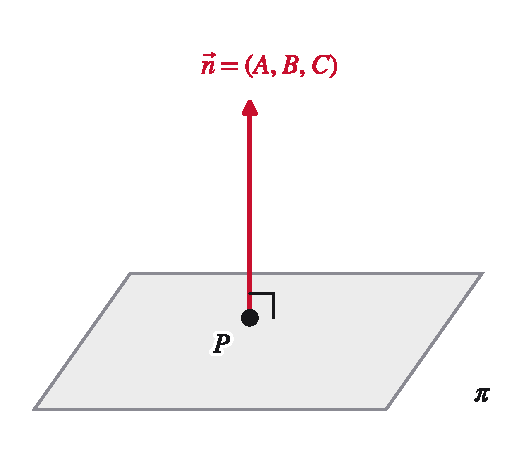
\includegraphics[width=248pt]{fig/m09_f18.pdf}
\caption{El vector normal $\vec n = (A, B, C)$ és perpendicular al pla $Ax + By + Cz + D = 0$.}
\end{figure}

\section{Recta determinada per dos plans}

La intersecció de dos plans no paral\textperiodcentered{}lels determina una recta:

\begin{equation*}
r: \begin{cases} Ax + By + Cz + D = 0 \\ A'x + B'y + C'z + D' = 0 \end{cases}
\end{equation*}

Perquè els dos plans determinin una recta cal que siguin no paral\textperiodcentered{}lels, és a dir, que els seus vectors normals $\vec n_1 = (A, B, C)$ i $\vec n_2 = (A', B', C')$ no siguin proporcionals. El vector director de la recta resultant és $\vec u = \vec n_1 \times \vec n_2$.

\section{Feix de plans}

\textbf{Definició:} El \textbf{feix de plans} és el conjunt de tots els plans que contenen (o passen per) una mateixa recta $r$. El vector normal de cadascun dels plans del feix és perpendicular a $r$.

Si la recta $r$ és la intersecció dels plans $\pi_1: A_1x + B_1y + C_1z + D_1 = 0$ i $\pi_2: A_2x + B_2y + C_2z + D_2 = 0$, qualsevol pla del feix es pot expressar com:

\begin{equation*}
\lambda\,(A_1x + B_1y + C_1z + D_1) + \mu\,(A_2x + B_2y + C_2z + D_2) = 0, \qquad (\lambda, \mu) \neq (0, 0)
\end{equation*}

\section{Complement: mètode per obtenir equacions}

\subsection{Recta per dos punts}

Per a la recta que passa per $A$ i $B$: es pren $A$ com a punt i $\vec d=\overrightarrow{AB}$ com a vector director.

\emph{Exemple:} Recta per $A(1,2,3)$ i $B(3,0,4)$. Vector director $\vec d=(2,-2,1)$.

\begin{equation*}
\begin{cases}x=1+2t\\y=2-2t\\z=3+t\end{cases}\qquad\Longleftrightarrow\qquad\frac{x-1}{2}=\frac{y-2}{-2}=\frac{z-3}{1}
\end{equation*}

\subsection{Pla per tres punts}

Es prenen dos vectors del pla, $\overrightarrow{AB}$ i $\overrightarrow{AC}$; el vector normal és el seu producte vectorial, i amb ell s'escriu $Ax+By+Cz+D=0$ imposant que passi per $A$.

\emph{Exemple:} Pla per $A(1,0,0)$, $B(0,1,0)$ i $C(0,0,1)$. $\overrightarrow{AB}=(-1,1,0)$ i $\overrightarrow{AC}=(-1,0,1)$, i

\begin{equation*}
\vec n=\overrightarrow{AB}\times\overrightarrow{AC}=(1,1,1)\;\Rightarrow\;x+y+z+D=0,\ \ A\in\pi\Rightarrow D=-1
\end{equation*}

El pla és $\pi:\ x+y+z-1=0$.

\emph{Alternativa:} $\begin{vmatrix}x-1&y&z\\-1&1&0\\-1&0&1\end{vmatrix}=0$ dóna el mateix pla.

\subsection{Passar d'una forma a una altra}

\textbf{De contínua a implícita} (dos plans). Se separen les igualtats de dues en dues.

\emph{Exemple:} $\dfrac{x-1}{2}=\dfrac{y+1}{-1}=\dfrac{z}{3}$.

\begin{itemize}
\item Primera i segona: $-(x-1)=2(y+1)\Rightarrow x+2y+1=0$.
\item Segona i tercera: $3(y+1)=-z\Rightarrow 3y+z+3=0$.
\end{itemize}

\begin{equation*}
r:\ \begin{cases}x+2y+1=0\\3y+z+3=0\end{cases}
\end{equation*}

\textbf{De implícita a paramètrica.} Es resol el sistema prenent una incògnita com a paràmetre.

\emph{Exemple:} $\begin{cases}x+y-z=1\\2x-y+z=2\end{cases}$. Sumant: $3x=3\Rightarrow x=1$. Llavors $y-z=0$; prenem $z=t$ i $y=t$.

\begin{equation*}
r:\ (x,y,z)=(1,0,0)+t\,(0,1,1)
\end{equation*}

\emph{Un cop tens un punt i un vector director, tens tot el que cal per al tema 10 i 11.}

\tema{10}{Posició relativa de rectes i plans}\section{Posició relativa de dos plans}

Donats dos plans $\pi: Ax + By + Cz + D = 0$ i $\pi': A'x + B'y + C'z + D' = 0$, la posició relativa es determina comparant els coeficients:

\begin{table}[H]
\centering
\renewcommand{\arraystretch}{1.25}
\begin{tabularx}{\textwidth}{lc>{\raggedright\arraybackslash}X}
\toprule
Plans coincidents & Plans paral\textperiodcentered{}lels & Plans secants \\
\midrule
$\dfrac{A}{A'} = \dfrac{B}{B'} = \dfrac{C}{C'} = \dfrac{D}{D'}$ & $\dfrac{A}{A'} = \dfrac{B}{B'} = \dfrac{C}{C'} \neq \dfrac{D}{D'}$ & No hi ha proporcionalitat entre els coeficients. La intersecció és una recta $r$. \\
\bottomrule
\end{tabularx}
\end{table}

\begin{figure}[H]
\centering
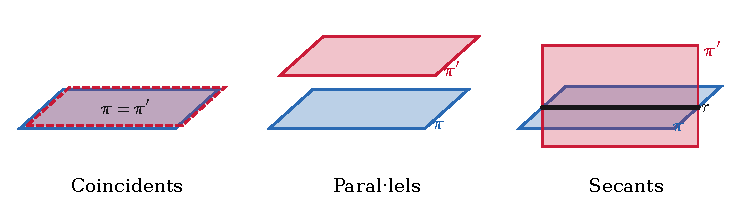
\includegraphics[width=372pt]{fig/m10_f19.pdf}
\caption{Posició relativa de dos plans: coincidents, paral\textperiodcentered{}lels i secants.}
\end{figure}

\section{Posició relativa de tres plans}

Amb tres plans, s'aplica el \textbf{Teorema de Rouché-Frobenius} sobre la matriu de coeficients $M$ i la matriu ampliada $M'$:

\begin{table}[H]
\centering
\renewcommand{\arraystretch}{1.25}
\begin{tabularx}{\textwidth}{lc>{\raggedright\arraybackslash}Xc}
\toprule
$\operatorname{Rg}(M)$ & $\operatorname{Rg}(M')$ & Posició relativa & Tipus \\
\midrule
1 & 1 & Tres plans coincidents & S.C.I \\
1 & 2 & Tres plans paral\textperiodcentered{}lels & S.I \\
2 & 2 & Tres plans secants a una recta $r$ comú & S.C.I \\
2 & 2 & Dos plans coincidents, l'altre secant als dos & S.C.I \\
2 & 3 & Prisma: plans secants dos a dos & S.I \\
2 & 3 & Dos plans paral\textperiodcentered{}lels, l'altre secant als dos & S.I \\
3 & 3 & Triedre: tres plans secants a un punt & S.C.D \\
\bottomrule
\end{tabularx}
\end{table}

\section{Posició relativa de recta i pla}

Per estudiar la posició de la recta $r$ i el pla $\pi$, es substitueixen les equacions paramètriques de $r$ a l'equació de $\pi$ i s'analitza el sistema resultant:

\begin{table}[H]
\centering
\renewcommand{\arraystretch}{1.25}
\begin{tabularx}{\textwidth}{>{\raggedright\arraybackslash}X>{\raggedright\arraybackslash}X>{\raggedright\arraybackslash}X}
\toprule
S.C.D & S.C.I & S.I \\
\midrule
$r$ i $\pi$ tenen un punt en comú (recta \textbf{secant} al pla) & $r$ està \textbf{continguda} en $\pi$ & $r$ i $\pi$ no tenen cap punt en comú (recta \textbf{paral\textperiodcentered{}lela} al pla) \\
\bottomrule
\end{tabularx}
\end{table}

\begin{figure}[H]
\centering
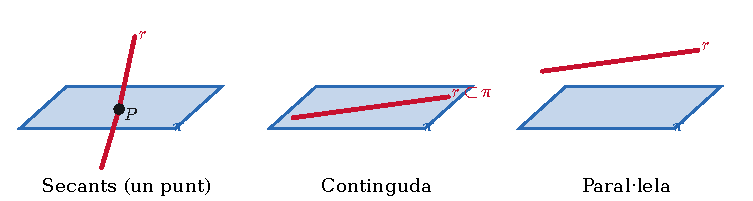
\includegraphics[width=372pt]{fig/m10_f20.pdf}
\caption{Les tres posicions relatives d'una recta i un pla.}
\end{figure}

\section{Posició relativa de dues rectes}

Expressades $r$ i $s$ com a intersecció de dos plans cadascuna, es forma un sistema de quatre equacions. Aplicant el TRF sobre la matriu $M$ i l'ampliada $M'$:

\begin{table}[H]
\centering
\renewcommand{\arraystretch}{1.25}
\begin{tabular}{lccc}
\toprule
S.C.D & S.C.I & S.I (1) & S.I (2) \\
\midrule
$\operatorname{Rg}(M) = 3 = \operatorname{Rg}(M')$ & $\operatorname{Rg}(M) = 2 = \operatorname{Rg}(M')$ & $\operatorname{Rg}(M) = 2 \neq \operatorname{Rg}(M') = 3$ & $\operatorname{Rg}(M) = 3 \neq \operatorname{Rg}(M') = 4$ \\
Rectes \textbf{secants} & Rectes \textbf{coincidents} & Rectes \textbf{paral\textperiodcentered{}leles} & Rectes que \textbf{s'encreuen} \\
\bottomrule
\end{tabular}
\end{table}

\subsection{Resum per vectors directors}

Donats els vectors directors $\vec u$ i $\vec v$ de $r$ i $s$, i el vector $\overrightarrow{PQ}$ entre un punt de cada recta:

\begin{itemize}
\item Si $\vec u = \lambda\vec v$ (vectors proporcionals, rectes paral\textperiodcentered{}leles o coincidents):
\begin{itemize}
\item $\overrightarrow{PQ} = \mu\,\vec u \Rightarrow$ rectes \textbf{coincidents}
\item $\overrightarrow{PQ} \neq \mu\,\vec u \Rightarrow$ rectes \textbf{paral\textperiodcentered{}leles}
\end{itemize}
\item Si $\vec u \neq \lambda\vec v$ (vectors no proporcionals):
\begin{itemize}
\item $D(\vec u, \vec v, \overrightarrow{PQ}) = 0 \Rightarrow$ rectes \textbf{secants}
\item $D(\vec u, \vec v, \overrightarrow{PQ}) \neq 0 \Rightarrow$ rectes que \textbf{s'encreuen}
\end{itemize}
\end{itemize}

on $D(\vec u, \vec v, \overrightarrow{PQ})$ és el determinant format per les tres files $\vec u$, $\vec v$ i $\overrightarrow{PQ}$.

\section{Perpendicularitat}

\subsection{Plans perpendiculars}

Dos plans $\pi_1$ i $\pi_2$ amb vectors normals $\vec n = (A, B, C)$ i $\vec n' = (A', B', C')$ són perpendiculars si:

\begin{equation*}
\vec n\cdot\vec n' = 0 \;\Longrightarrow\; AA' + BB' + CC' = 0
\end{equation*}

\subsection{Recta i pla perpendiculars}

Una recta de vector director $\vec v = (V_1, V_2, V_3)$ és perpendicular al pla $Ax + By + Cz + D = 0$ si $\vec v$ és proporcional al vector normal $\vec n = (A, B, C)$:

\begin{equation*}
\vec v = k\,\vec n,\; k \neq 0 \iff \frac{V_1}{A} = \frac{V_2}{B} = \frac{V_3}{C}
\end{equation*}

\subsection{Rectes perpendiculars}

Dues rectes amb vectors directors $\vec v$ i $\vec u$ són perpendiculars si:

\begin{equation*}
\vec v\cdot\vec u = 0
\end{equation*}

\section{Projeccions ortogonals sobre un pla}

\subsection{Projecció ortogonal d'un punt sobre un pla}

El punt $P'$ és la \textbf{projecció ortogonal} de $P$ sobre el pla $\pi$ si $P'$ és el peu de la perpendicular a $\pi$ que passa per $P$. Es troba com la intersecció de $\pi$ amb la recta perpendicular a $\pi$ que passa per $P$.

\begin{figure}[H]
\centering
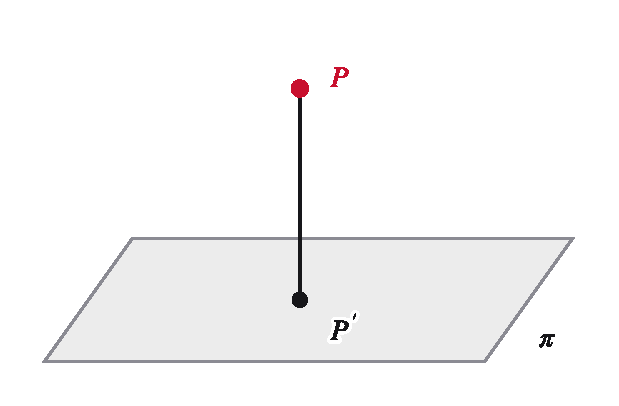
\includegraphics[width=297pt]{fig/m10_f21.pdf}
\caption{Projecció ortogonal del punt $P$ sobre el pla $\pi$: el punt $P'$ és el peu de la perpendicular.}
\end{figure}

\subsection{Projecció ortogonal d'una recta sobre un pla}

La projecció ortogonal d'una recta $r$ sobre un pla $\pi$ és la recta $r'$ que resulta d'intersectar $\pi$ amb el pla que conté $r$ i és perpendicular a $\pi$. Per a un segment $PQ$, es projecten els extrems $P$ i $Q$ per obtenir $P'$ i $Q'$.

\subsection{Projecció ortogonal d'un punt sobre una recta}

La projecció ortogonal del punt $P$ sobre la recta $r$ és el punt $P'$ intersecció de $r$ amb el pla perpendicular a $r$ que passa per $P$. El vector normal d'aquest pla coincideix amb el vector director de $r$.

\tema{11}{Distàncies i angles}\section{Distància entre dos punts}

Donats $P = (x_1, y_1, z_1)$ i $Q = (x_2, y_2, z_2)$, la distància és el mòdul del vector $\overrightarrow{PQ}$:

\begin{equation*}
d(P, Q) = |\overrightarrow{PQ}| = \sqrt{(x_2 - x_1)^2 + (y_2 - y_1)^2 + (z_2 - z_1)^2}
\end{equation*}

\section{Distància d'un punt a una recta}

La distància entre el punt $P$ i la recta $r$ és $d(P, r) = d(P, P')$, on $P'$ és la projecció ortogonal de $P$ sobre $r$. Es pot calcular de dues maneres:

\begin{enumerate}
\item \textbf{Mètode geomètric:} trobar $P'$ (intersecció del pla $\perp r$ per $P$ amb $r$) i calcular $d(P, P')$.
\item \textbf{Mitjançant el producte vectorial} (si $\vec u$ és el vector director de $r$ i $Q \in r$):
\end{enumerate}

\begin{equation*}
d(P, r) = \frac{|\vec u\times\overrightarrow{QP}|}{|\vec u|}
\end{equation*}

\begin{figure}[!htbp]
\centering
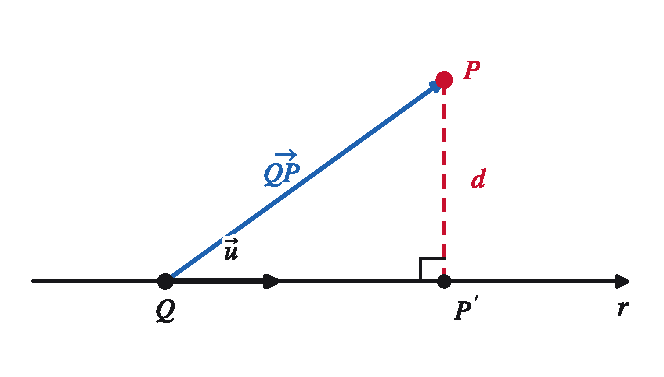
\includegraphics[width=319pt]{fig/m11_f22.pdf}
\caption{Distància del punt $P$ a la recta $r$: $d = |\vec u\times\overrightarrow{QP}|\,/\,|\vec u|$.}
\end{figure}

\section{Distància d'un punt a un pla}

La distància del punt $P(x_0, y_0, z_0)$ al pla $\pi: Ax + By + Cz + D = 0$ és $d(P, \pi) = d(P, P')$, on $P'$ és el peu de la perpendicular. La fórmula directa és:

\begin{equation*}
d(P, \pi) = \frac{|Ax_0 + By_0 + Cz_0 + D|}{\sqrt{A^2 + B^2 + C^2}}
\end{equation*}

\begin{figure}[!htbp]
\centering
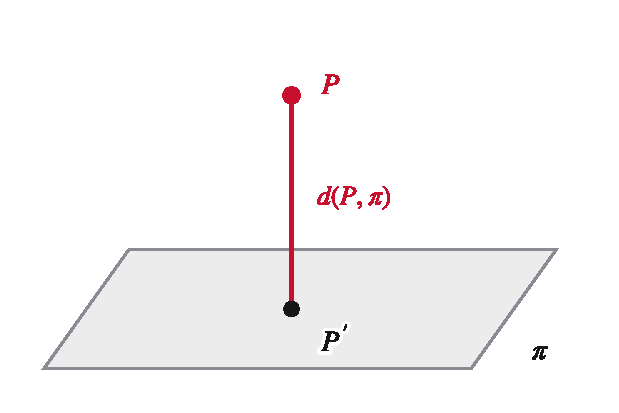
\includegraphics[width=297pt]{fig/m11_f23.pdf}
\caption{Distància del punt $P$ al pla $\pi$: la longitud del segment perpendicular a $\pi$ que passa per $P$.}
\end{figure}

\section{Distàncies entre rectes i plans}

\subsection{Distància entre dues rectes}

\begin{itemize}
\item \textbf{Secants o coincidents:} $d = 0$.
\item \textbf{Paral\textperiodcentered{}leles:} $d(r, s) = d(P, s)$, on $P$ és qualsevol punt de $r$.
\item \textbf{Que s'encreuen:} existeix una única recta $t$ perpendicular a ambdues. Si $P \in r$ i $P' \in s$ són els punts de contacte de $t$, aleshores $d(r, s) = d(P, P')$. Fórmula amb el producte mixt (apartat 8):
\end{itemize}

\begin{equation*}
d(r, s) = \frac{|[\overrightarrow{PQ}, \vec u, \vec v]|}{|\vec u\times\vec v|}
\end{equation*}

on $P \in r$, $Q \in s$, $\vec u$ i $\vec v$ són els vectors directors de $r$ i $s$.

\subsection{Distància entre una recta i un pla}

\begin{itemize}
\item Si la recta talla el pla o hi és continguda: $d = 0$.
\item Si la recta és paral\textperiodcentered{}lela al pla: $d(r, \pi) = d(P, \pi)$, on $P$ és qualsevol punt de $r$.
\end{itemize}

\subsection{Distància entre dos plans}

\begin{itemize}
\item Si es tallen o són coincidents: $d = 0$.
\item Si són paral\textperiodcentered{}lels: $d(\pi_1, \pi_2) = d(P, \pi_2)$, on $P$ és qualsevol punt de $\pi_1$.
\end{itemize}

\section{Angles formats per rectes i plans}

L'angle entre dos vectors $\vec v$ i $\vec w$ és:

\begin{equation*}
\vec v\cdot\vec w = |\vec v|\,|\vec w|\cos\alpha \;\Longrightarrow\; \alpha = \arccos\frac{\vec v\cdot\vec w}{|\vec v|\,|\vec w|}
\end{equation*}

\subsection{Angle entre dues rectes}

L'angle format per $r$ i $s$ és el més petit dels angles formats pels seus vectors directors $\vec u$ i $\vec v$ (es pren valor absolut per garantir un angle agut):

\begin{equation*}
\cos\alpha = \frac{|\vec u\cdot\vec v|}{|\vec u|\,|\vec v|} \;\Rightarrow\; \alpha = \arccos\frac{|\vec u\cdot\vec v|}{|\vec u|\,|\vec v|}
\end{equation*}

\subsection{Angle entre una recta i un pla}

L'angle $\alpha$ entre la recta $r$ (vector director $\vec u$) i el pla $\pi$ (vector normal $\vec n$) és el complement de l'angle $\beta$ entre $\vec u$ i $\vec n$:

\begin{equation*}
\sin\alpha = \cos\beta = \frac{|\vec u\cdot\vec n|}{|\vec u|\,|\vec n|} \;\Rightarrow\; \alpha = \arcsin\frac{|\vec u\cdot\vec n|}{|\vec u|\,|\vec n|}
\end{equation*}

\begin{figure}[!htbp]
\centering
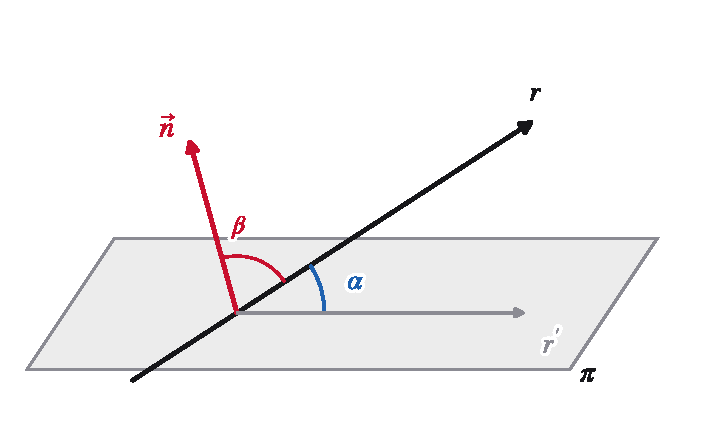
\includegraphics[width=341pt]{fig/m11_f24.pdf}
\caption{Angle $\alpha$ entre la recta $r$ i el pla $\pi$: $\sin\alpha = \cos\beta = |\vec u\cdot\vec n|\,/\,(|\vec u||\vec n|)$.}
\end{figure}

\subsection{Angle entre dos plans}

L'angle entre $\pi_1$ i $\pi_2$ (amb vectors normals $\vec n_1$ i $\vec n_2$) és el més petit dels angles diedres:

\begin{equation*}
\cos\alpha = \frac{|\vec n_1\cdot\vec n_2|}{|\vec n_1|\,|\vec n_2|} \;\Rightarrow\; \alpha = \arccos\frac{|\vec n_1\cdot\vec n_2|}{|\vec n_1|\,|\vec n_2|}
\end{equation*}

\section{Producte vectorial de dos vectors}

\textbf{Definició:} El \textbf{producte vectorial} de $\vec u = (u_1, u_2, u_3)$ i $\vec v = (v_1, v_2, v_3)$ és el vector

\begin{equation}
\vec u\times\vec v = \begin{vmatrix} \vec e_1 & u_1 & v_1 \\ \vec e_2 & u_2 & v_2 \\ \vec e_3 & u_3 & v_3 \end{vmatrix} = (u_2v_3 - u_3v_2,\; u_3v_1 - u_1v_3,\; u_1v_2 - u_2v_1)
\end{equation}

Les característiques del vector $\vec u\times\vec v$ són:

\begin{itemize}
\item \textbf{Mòdul:} $|\vec u\times\vec v| = |\vec u|\,|\vec v|\sin\alpha$, amb $0^\circ \le \alpha \le 180^\circ$.
\item \textbf{Direcció:} perpendicular als dos vectors $\vec u$ i $\vec v$.
\item \textbf{Sentit:} el d'avanç d'un tirabuixó que giri de $\vec u$ a $\vec v$ en el menor angle possible (regla de la mà dreta).
\end{itemize}

\emph{Observació:} si $\vec u\cdot\vec v = 0$, els vectors són perpendiculars i $|\vec u\times\vec v| = |\vec u|\,|\vec v|$ (valor màxim).

\section{Aplicacions geomètriques del producte vectorial}

\subsection{Àrea d'un paral\textperiodcentered{}lelogram}

Si $\vec u$ i $\vec v$ són dos costats adjacents del paral\textperiodcentered{}lelogram:

\begin{equation*}
A = |\vec u\times\vec v|
\end{equation*}

\subsection{Àrea d'un triangle}

Donats tres vèrtexs $P$, $Q$, $R$:

\begin{equation*}
A = \frac12\,|\overrightarrow{PQ}\times\overrightarrow{PR}|
\end{equation*}

\subsection{Distància d'un punt a una recta (forma alternativa)}

Si $Q \in r$ i $\vec u$ és el vector director de $r$:

\begin{equation*}
d(P, r) = \frac{|\vec u\times\overrightarrow{QP}|}{|\vec u|}
\end{equation*}

\section{Producte mixt de tres vectors}

\textbf{Definició:} El \textbf{producte mixt} dels vectors $\vec u$, $\vec v$ i $\vec w$ és el nombre real

\begin{equation}
[\vec u, \vec v, \vec w] = \vec u\cdot(\vec v\times\vec w) = \begin{vmatrix} u_1 & u_2 & u_3 \\ v_1 & v_2 & v_3 \\ w_1 & w_2 & w_3 \end{vmatrix}
\end{equation}

\section{Aplicacions geomètriques del producte mixt}

\subsection{Volum d'un paral\textperiodcentered{}lelepípede}

Si $\vec u$, $\vec v$ i $\vec w$ són tres arestes adjacents:

\begin{equation*}
V = |[\vec u, \vec v, \vec w]|
\end{equation*}

\subsection{Volum d'una piràmide de base triangular}

\begin{equation*}
V = \frac16\,|[\vec u, \vec v, \vec w]|
\end{equation*}

\subsection{Distància entre dues rectes que s'encreuen}

Si $P \in r$, $Q \in s$, i $\vec u$, $\vec v$ són els vectors directors de $r$ i $s$:

\begin{equation*}
|[\overrightarrow{PQ}, \vec u, \vec v]| = |\vec u\times\vec v|\cdot d(r, s) \;\Longrightarrow\; d(r, s) = \frac{|[\overrightarrow{PQ}, \vec u, \vec v]|}{|\vec u\times\vec v|}
\end{equation*}

\section{Complement: punts i figures simètriques}

\subsection{Mètode general}

El \textbf{simètric} $P'$ d'un punt $P$ respecte d'un element (punt, recta o pla) es troba trobant primer el \textbf{punt mitjà} $M$ entre $P$ i $P'$ i després aïllant:

\begin{equation*}
M=\frac{P+P'}{2}\quad\Longrightarrow\quad P'=2M-P
\end{equation*}

\begin{table}[!htbp]
\centering
\renewcommand{\arraystretch}{1.3}
\begin{tabularx}{\textwidth}{l>{\raggedright\arraybackslash}X}
\toprule
Respecte de\ldots{} & Com trobar $M$ \\
\midrule
un punt $Q$ & $M=Q$ \\
una recta $r$ & $M=r\cap\pi$, on $\pi$ és el pla per $P$ \textbf{perpendicular} a $r$ (vector normal $=\vec d_r$) \\
un pla $\pi$ & $M=r\cap\pi$, on $r$ és la recta per $P$ \textbf{perpendicular} a $\pi$ (vector director $=\vec n_\pi$) \\
\bottomrule
\end{tabularx}
\end{table}

\begin{figure}[!htbp]
\centering
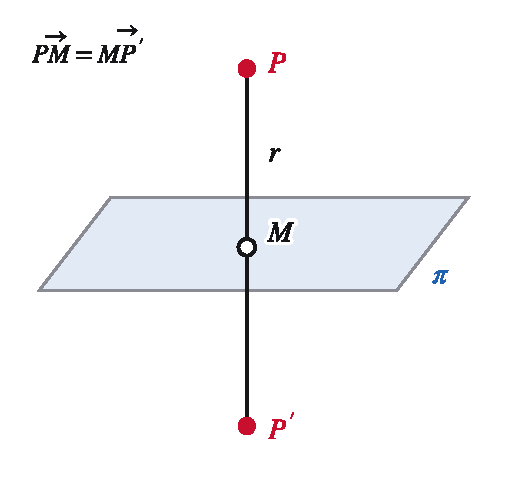
\includegraphics[width=251pt]{fig/m11_f37.pdf}
\caption{El simètric $P'$ de $P$ respecte d'un pla: $M$ és la intersecció de la perpendicular $r$ amb el pla i és el punt mitjà de $PP'$.}
\end{figure}

\subsection{Exemple 1 --- Simètric respecte d'un pla}

Simètric de $P(1,2,3)$ respecte de $\pi:\ x+y+z-3=0$.

\begin{enumerate}
\item Recta perpendicular per $P$: $r:\ (1+t,\,2+t,\,3+t)$.
\item Intersecció amb $\pi$: $(1+t)+(2+t)+(3+t)-3=0\Rightarrow 3+3t=0\Rightarrow t=-1$, de manera que $M=(0,1,2)$.
\item $P'=2M-P=(2\cdot0-1,\,2\cdot1-2,\,2\cdot2-3)=(-1,0,1)$.
\end{enumerate}

\emph{Comprovació:} $-1+0+1-3=-3$ i $1+2+3-3=3$: estan a banda i banda del pla i a la mateixa distància $\checkmark$.

\subsection{Exemple 2 --- Simètric respecte d'una recta}

Simètric de $P(1,2,0)$ respecte de $r:\ (t,\,t,\,0)$ amb $\vec d=(1,1,0)$.

\begin{enumerate}
\item Pla per $P$ perpendicular a $r$: $x+y+D=0$ i $1+2+D=0\Rightarrow D=-3$, així que $\pi:\ x+y-3=0$.
\item $M=r\cap\pi$: $t+t-3=0\Rightarrow t=\frac32$ i $M=\left(\frac32,\frac32,0\right)$.
\item $P'=2M-P=(3-1,\,3-2,\,0)=(2,1,0)$.
\end{enumerate}

\subsection{Pla mediador}

El \textbf{pla mediador} d'un segment $AB$ és el pla perpendicular a $AB$ pel seu punt mitjà: conté tots els punts equidistants d'$A$ i $B$.

\emph{Exemple:} $A(1,0,2)$ i $B(3,2,0)$. $\overrightarrow{AB}=(2,2,-2)\parallel(1,1,-1)$ i $M=(2,1,1)$. Llavors $x+y-z+D=0$ amb $2+1-1+D=0\Rightarrow D=-2$:

\begin{equation*}
\pi:\ x+y-z-2=0
\end{equation*}

\section{Complement: interpretació geomètrica dels productes vectorial i mixt}

\begin{figure}[!htbp]
\centering
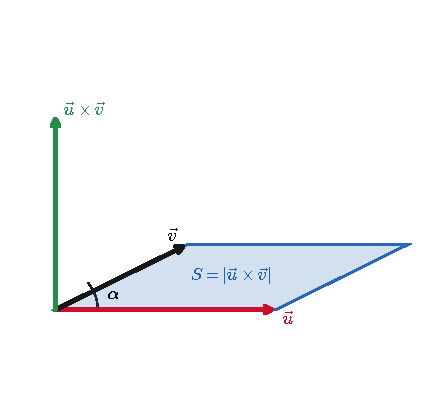
\includegraphics[width=208pt]{fig/x11_cross.pdf}
\caption{El producte vectorial $\vec u\times\vec v$ és perpendicular al pla que formen $\vec u$ i $\vec v$ (regla de la mà dreta) i el seu mòdul és l'àrea del paral\textperiodcentered{}lelogram.}
\end{figure}

El sentit de $\vec u\times\vec v$ es determina amb la \textbf{regla de la mà dreta}: si els dits van de $\vec u$ cap a $\vec v$ pel camí més curt, el polze indica el sentit del producte. Per això $\vec v\times\vec u=-\,\vec u\times\vec v$.

\begin{figure}[!htbp]
\centering
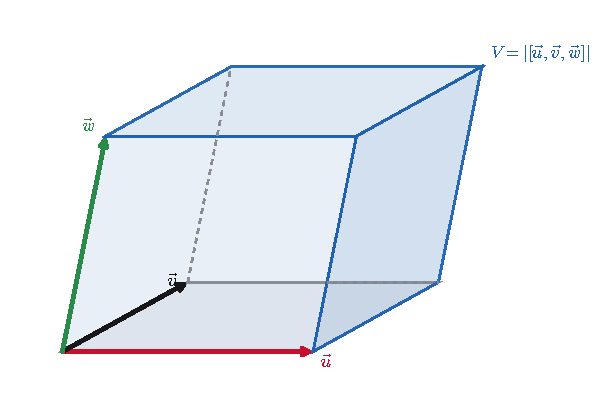
\includegraphics[width=286pt]{fig/x11_parallelepiped.pdf}
\caption{El valor absolut del producte mixt $[\vec u,\vec v,\vec w]$ és el volum del paral\textperiodcentered{}lelepípede definit pels tres vectors.}
\end{figure}

El producte mixt es calcula com a determinant: $[\vec u,\vec v,\vec w]=\begin{vmatrix}u_1&u_2&u_3\\v_1&v_2&v_3\\w_1&w_2&w_3\end{vmatrix}$. Si val $0$, els tres vectors són coplanaris.

\section{Complement: exemples resolts de distàncies, angles i volums}

\emph{Exemple 1 --- Distància d'un punt a un pla:} $P(1,2,3)$ i $\pi:\ 2x-y+2z-4=0$:

\begin{equation*}
d(P,\pi)=\frac{|2\cdot1-2+2\cdot3-4|}{\sqrt{2^2+(-1)^2+2^2}}=\frac{2}{3}.
\end{equation*}

\emph{Exemple 2 --- Distància entre dues rectes que s'encreuen:} $r:(0,0,0)+t(1,0,0)$ i $s:(0,1,0)+u(0,0,1)$. $\vec u\times\vec v=(0,-1,0)$, $\overrightarrow{PQ}=(0,1,0)$ i $[\vec u,\vec v,\overrightarrow{PQ}]=-1$:

\begin{equation*}
d(r,s)=\frac{|[\vec u,\vec v,\overrightarrow{PQ}]|}{|\vec u\times\vec v|}=\frac11=1.
\end{equation*}

\emph{Exemple 3 --- Angle entre dos plans:} $\pi:x+y+z=0$ i $\pi':x+y=0$, amb $\vec n=(1,1,1)$ i $\vec n'=(1,1,0)$:

\begin{equation*}
\cos\alpha=\frac{|\vec n\cdot\vec n'|}{|\vec n|\,|\vec n'|}=\frac{2}{\sqrt3\,\sqrt2}=\frac{2}{\sqrt6}\ \Rightarrow\ \alpha\approx35{,}3^{\circ}.
\end{equation*}

\emph{Exemple 4 --- Angle entre una recta i un pla:} $r$ de vector director $\vec u=(1,2,2)$ i el pla $z=0$ ($\vec n=(0,0,1)$): $\sin\alpha=\dfrac{|\vec u\cdot\vec n|}{|\vec u|\,|\vec n|}=\dfrac23\Rightarrow\alpha\approx41{,}8^{\circ}$.

\emph{Exemple 5 --- Àrea d'un triangle i volum d'un tetraedre:} Siguin $A(1,0,0)$, $B(0,2,0)$, $C(0,0,3)$ i $O(0,0,0)$.

\begin{itemize}
\item $\overrightarrow{AB}=(-1,2,0)$ i $\overrightarrow{AC}=(-1,0,3)$; $\overrightarrow{AB}\times\overrightarrow{AC}=(6,3,2)$ amb mòdul $7$. Àrea del triangle $ABC=\dfrac72$.
\item El volum del tetraedre $OABC$ és $\dfrac16\bigl|[\overrightarrow{OA},\overrightarrow{OB},\overrightarrow{OC}]\bigr|=\dfrac16\cdot6=1$.
\item El pla $ABC$ és $\dfrac x1+\dfrac y2+\dfrac z3=1$, és a dir, $6x+3y+2z-6=0$, i la distància d'$O$ a aquest pla és $\dfrac{6}{7}$. Comprovació: $V=\dfrac13\cdot\dfrac72\cdot\dfrac67=1$.
\end{itemize}

\emph{Exemple 6 --- Distància d'un punt a una recta:} $P(1,1,1)$ i $r:(0,0,0)+t(1,0,0)$. $\overrightarrow{QP}=(1,1,1)$ i $\vec u\times\overrightarrow{QP}=(0,-1,1)$, de mòdul $\sqrt2$: $d(P,r)=\dfrac{\sqrt2}{1}=\sqrt2$.


\end{document}
